% Title page.
\title[Aula 03]{Oceanografia Física Dinâmica}
\subtitle{Conceitos de Dinâmica de Fluidos Geofísicos}
\author[Filipe Fernandes]{Filipe P. A. Fernandes}
\institute[unimonte]{Centro Universitário Monte Serrat}
\date[Fevereiro 2014]{24 de Fevereiro 2014}

\logo{
\includegraphics[scale=0.15]{../common/university_logo.png}}

\begin{document}

% The title page frame.
\begin{frame}[plain]
  \titlepage
\end{frame}

\section*{Outline}
\begin{frame}
\frametitle{Índice}
\tableofcontents
\end{frame}

\section{Forças de Volume: forças de atração gravitacional e Coriolis, referencial inercial e referencial não inercial.}

\subsection{Recapitulando...}
\begin{frame}
\frametitle{Recapitulando... (quadro 01)}
  \begin{center}
    \shadowbox{\includegraphics[scale=0.5]{./figures/coordinates.png}}
  \end{center}
\end{frame}

\subsection{Forças de volume: força de atração gravitacional.}
\begin{frame}
\frametitle{Força de atração gravitacional (quadro 02)}
  \begin{center}
    \shadowbox{\includegraphics[scale=0.7]{./figures/gravity.png}}
  \end{center}
\end{frame}

\subsection{Forças de volume: força de Coriolis}
\begin{frame}
\frametitle{Força de Coriolis (quadro 03)}
  \begin{center}
    \shadowbox{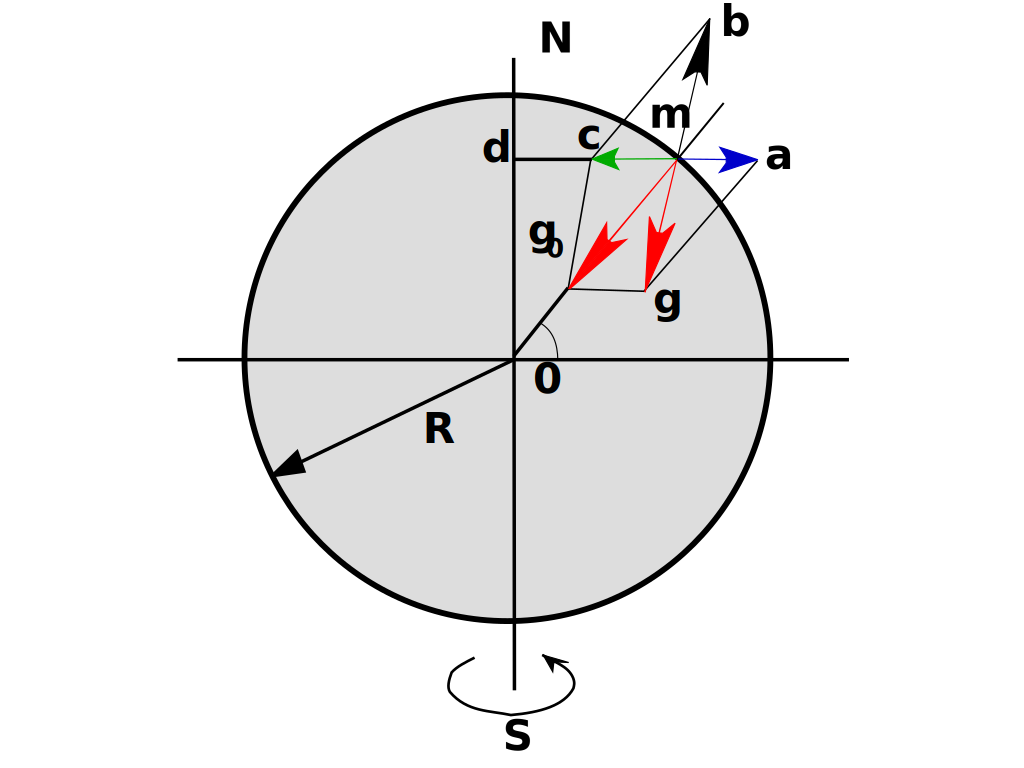
\includegraphics[scale=0.3]{./figures/Earth_Rotation.png}}
  \end{center}
  {\scriptsize \url{http://en.wikipedia.org/wiki/Foucault_pendulum}}
\end{frame}

\begin{frame}
\frametitle{Dever de casa -- 03}
  \begin{block}{}
    Exercício prático -- 01
  \end{block}
\end{frame}


\end{document}
